\chapter{Resilience of Deep Aquifer Microbial Communities to Seasonal Hydrological Fluctuations}
\label{ch:microbiology}

% ------------ 1st page ------------- %

\chaptermark{Chapter 3} % to change the headers
%\setcounter{figure}{0}
%\setcounter{table}{0}

Sébastien Giroud$^{1,2}$, Longhui Deng$^{3}$, Mark A. Lever$^{2,4}$, 
Oliver S. Schilling$^{1,5}$, and Rolf Kipfer$^{1,2,6}$ \\

\noindent
This chapter has been published in \textit{}.\\
DOI: \url{}

\blfootnote{\begin{flushleft}
$^{1}$Department of Water Resources and Drinking Water, Eawag, Dübendorf, Switzerland\\
$^{2}$Institute of Biogeochemistry and Pollutant Dynamics, ETH Zürich, Zurich, Switzerland\\
$^{3}$School of Oceanography, Shanghai Jiao Tong University, Shanghai, China\\
$^{4}$Department of Marine Science, University of Texas at Austin, Port Aransas, USA\\
$^{5}$Hydrogeology, Department of Environmental Sciences, University of Basel, Basel, Switzerland\\
$^{6}$Institute of Geochemistry and Petrology, ETH Zürich, Zurich, Switzerland\\
\end{flushleft}}

\vspace*{\fill}
\null{
\textcolor{gray}{
\footnotesize % Adjust size as needed
\noindent
\textbf{Acknowledgements}\\ 
We thank Gabriele Bianchetti, Alpgeo and Cesla to allow us access to the wells facilities and to provide us geochemical data.
We acknowledge Madalina Jagger, Caroline Stengel, and Serge Robert for the isotopic measurements at ETH Zurich and Eawag, and Clemens Glombitza for the measurements of volatile fatty acids.
We thank the entire team of the Tracer Hydrogeology, Environmental Isotopes and former Environmental Microbiology groups at Eawag and ETH Zurich for their help and insightful discussions.
PhD support for SG and open access funding provided by Eawag – Swiss Federal Institute of Aquatic Science and Technology, with additional financial support from the Canton of Valais.
OSS gratefully acknowledges the funding received through SNSF-JSPS SJSSTP grant 214048.
Microbiologic data produced and analyzed in this paper were generated in collaboration with the Genetic Diversity Centre (GDC), ETH Zurich.
We sincerely thank the two reviewers for their constructive feedback, which helped improve the manuscript, and the editor for handling our submission.
}}

% ------------ 2nd page ------------- %
\newpage
\noindent
\textbf{Abstract:} The influence of seasonal variations in temperature and precipitation on subsurface biogeochemical processes remains poorly understood.
In the Lavey-les-Bains thermal system in the Swiss Alps, annual variations in electrical conductivity are observed to depths of \SI{500}{\metre}, suggesting a potential link to surface environmental changes.
Here we show, through year-round analyses of stable water isotopes, noble gases and conductivity, that seasonally varying contributions of shallow groundwater from the Rhône alluvial aquifer mix with deep groundwater.
Despite vertically similar fluid geochemical compositions suggesting high hydrological connectivity, microbial communities exhibit significant depth-dependent variation with minimal seasonal change.
This decoupling of dynamic water source partitioning and stable microbial community structure has not been previously observed and fills a critical gap in our understanding of geothermal systems and microbial life in the deep subsurface.
At \SI{200}{\metre}, the communities are dominated by sulfur-disproportionating Bacteria (\textit{Dissulfurispira}) and Micrarchaeota, while at \SI{500}{\metre} the major groups include sulfate- and iron-reducers and/or hydrogen-oxidizers (Thermales, Thermodesulfobacteriota, and Bathyarchaeota).
Our study highlights the resilience of terrestrial subsurface microbial communities to temporal variations in water sources and fluid composition.
We propose that intrinsic environmental properties---such as temperature---are more critical drivers of microbial community structure in hydrologically connected deep aquifers than seasonal hydrological changes.

\section{Introduction}
eothermal water resources are increasingly recognized not only for their traditional therapeutic and recreational benefits but also for their potential to address contemporary energy challenges \citep{kagel2005guide}.
As global efforts intensify to mitigate climate change, the sustainable heat derived from the Earth’s crust is vital for both direct thermal heating and geothermal power generation, offering a solution to offset greenhouse gas emissions \citep{fridleifsson2008possible}. 
Additionally, these waters are often enriched in critical raw materials such as lithium and helium (He) \citep{harrison2014technologies, simmons2018strategic}.
This multifaceted utility of geothermal resources positions them at the intersection of health, energy, and mineral resources sectors, highlighting their broad relevance in a transitioning energy landscape.

Despite the growing utility of geothermal resources, our understanding of deep hot aquifers, especially the interconnections between geochemistry, heat, and the deep biosphere, remains limited particularly in continental systems. 
Accessing these remote environments poses significant challenges due to their depth and geological complexity. 
Like all groundwater systems, the temporal evolution of thermal groundwater is influenced by the dynamics of recharge, transport, mixing, and discharge. 
These processes enable the use of environmental tracers, which provide valuable insights into the evolution and characteristics of these geothermal resources.

Environmental tracers are pivotal in characterizing groundwater re-gimes across various applications.
These tracers, whether introduced artificially or inherent within the groundwater, are essential for mapping flow paths using breakthrough curves.
Electrical conductivity measurements, for instance, help pinpoint water origins \citep{plummer2000age} and have the potential to track geochemical transformations \citep{mengis1999multiple}.
Similarly, the isotopic composition of water (\ce{^3H}, $\delta$\ce{^2H} and $\delta$\ce{^{18}O}) provides insights into groundwater origins and residence time, as well as seasonality and altitude of recharge that feeds groundwater systems, enabling a better understanding of their recharge mechanisms \citep{blasch2007distinguishing}.
Analyzing water geochemistry, particularly ion concentrations, helps to characterize interactions between water and the surrounding rocks during its transport \citep{elango2007rock}.
Dissolved gases, along with their stable or radio-isotopic compositions, are moreover an effective tool for determining groundwater recharge times through helium, argon, and krypton dating methods \citep{kipfer2002noble}.
On the other hand, the occurrence and dynamics of reactive and biologically relevant gases, such as \ce{O2}, \ce{CH4}, and \ce{CO2}, indicate biotic and abiotic transformations occurring deep underground, particularly when concentration measurements are combined with isotopic analyses \citep{bottrell2019carbon, whiticar1999carbon}.
These measurements are crucial for investigating deep microbial communities within the Earth's crust and contribute to our understanding of biogeochemical cycles in these systems.

Substantial research has focused on subsurface marine sedimentary environments, where microbial communities primarily utilize ancient, photosynthetically produced organic matter as their energy source \citep{biddle2006heterotrophic, hondt2015presence, bradley2019survival}.
In contrast, less explored marine crustal and serpentinitic habitats are thought to support life forms dependent on endogenous \ce{H2} and \ce{CH4}, supporting microbial communities with lower diversity and biomass compared to sedimentary environments \citep{lever2013evidence, fruh2018magmatism, templeton2021accessing}, as well as rare, highly phylogenetically diverse communities near thermally active vents \citep{sogin2006microbial}.
Similarly, terrestrial subsurface environments, such as South African gold mines and Scandinavian granitic rocks, often reveal microbial communities with low diversity \citep{bomberg2015active, itavaara2011characterization, magnabosco2016metagenomic}, whereas volcanic environments exhibit more diverse microbial communities \citep{schilling2023revisiting, kato2009deep}.
These findings highlight the need for further exploration of deep crustal habitats to better understand the drivers of microbial diversity in deep continental environments.

The Rhône valley, nestled in the Swiss Alps, is recognized as one of Switzerland's most seismically active regions. 
The active tectonics led to the formation of geothermal systems, including Lavey-les-Bains. 
There, it is hypothesized that groundwater flows for millennia (about \SIrange{8000}{30000}{\year}, based on \ce{^{14}C} dating and particle tracking model) through the deep crystalline formations of the Aiguilles Rouges massif  \citep{bianchetti1994hydrogeologie, sonney2009numerical}.
The deep flow path allows water to heat up before ascending through a fractured rock system, ultimately reaching and mixing with shallower groundwater in the alluvial plains.
Remarkably, electrical conductivity has been observed to vary seasonally in the thermal wells feeding the spa \citep{sonney2009numerical}. 
This highlights the complex hydrological dynamics of the region, where shallow and deep groundwater feed and mix together in the thermal system of Lavey-les-Bains.

Lavey-les-Bains allow to study the hydrological and geomicrobiological dynamics of a thermal system at different depths, thanks to its extensive network of wells and the comprehensive hydrochemical data collected by the spa.
In this study, we investigate the drivers of seasonal groundwater mixing dynamics at Lavey-les-Bains and how these changes influence groundwater chemistry and in situ microbial communities.
To achieve this, we combine microbial eDNA analyses with quasi-continuous measurements of dissolved gases and other geochemical parameters in three thermal wells (P201: \SI{201}{\metre}, \SI{51}{\celsius}; P280: \SI{276}{\metre}, \SI{53}{\celsius}; P600: \SI{516}{\metre}, \SI{64}{\celsius}; Figure~\ref{figSI:map_Lavey}).
We investigate the major sources of groundwater and how seasonal variations in these sources affect the geochemical properties of the fluid and the microbial communities within the aquifer.
By integrating hydrological, geochemical and microbial data, our research elucidates the complex interplay between geological and biological processes in the geothermally active environment of Lavey-les-Bains.
This study provides unique insights into how deep microbial communities adapt to seasonal mixing dynamics.

%%%%%%%%%%%%%%%%%%%%%%%%%%%%%%%%%%%%%%%%%%%%%%%%%%%%%%%%%%%%%%%%%%%%%%%%%%%%%%%%%%%%%%%%%%%%%%%%%%%%%%%%%%%%

\section{Results}
\subsection{Geochemical data}
\subsubsection{Electrical Conductivity} 
Weekly measurements of electrical conductivity ($\kappa_{20}$ in \SI{}{\milli\siemens\per\centi\metre}) in wells P201 and P600 are in line with previous observations \citep{sonney2009numerical} and show distinctive seasonal patterns, with conductivity peaking between July and October and dipping from December to March (Figure~\ref{fig:season}).
The variability lies around \SIrange{10}{15}{\percent} for P600 and \SIrange{25}{30}{\percent} for P201.
Comparatively, P600 consistently exhibits higher conductivity than P201 during similar periods as would be expected for deeper and more evolved thermal water \citep{nono2020electrical}.
Although the amplitude of conductivity changes is less pronounced in P600 than in P201, suggesting a more hydrochemically stable environment at greater depths, the persistent seasonality indicates seasonally fluctuating hydrological conditions even at these depths.

\subsubsection{Hydrogeochemistry}
Biannual sampling of hydrogeochemical parameters (Table~\ref{table:geochemistry}, e.g., pH, inorganic anion and cation concentrations) classifies the thermal waters of the various wells at Lavey-les-Bains as sodium-chloride type, indicative of deep geothermal systems and often associated with high \ce{CO2} content \citep{gupta2007exploration}.
Notably, well P600 exhibits significantly higher \ce{Na+}, \ce{NH4+}, \ce{Li+}, \ce{Cl-}, \ce{S^{2-}}, \ce{SO4^{2-}}, and \ce{Si^{4+}} concentrations than well P201, while its \ce{Mg^{2+}} levels are comparatively lower (Figure~\ref{figSI:geochemistry}).
Well P280 exhibits ion concentrations that are similar to P600 for \ce{SO4^{2-}}, similar to P201 for \ce{Na+}, \ce{K+}, and \ce{Mg^{2+}}, and intermediate for other ions such as \ce{S^{2-}} and \ce{Ca^{2+}}.
This suggests that P280 might represent a transitional geochemical state between P201 and P600.
These vertical concentration gradients likely reflect depth-related changes in geochemical processes that are influenced by the geological formation through which the water travels and/or varying mixing dynamics between shallow and deep groundwater components.


\FloatBarrier % Ensure previous floats are placed before proceeding

\afterpage{% Delays the figure until the next page
\clearpage
\begin{table*}[ht]
\caption{Geochemical parameters in the three main deep wells of Lavey-les-Bains and the surface well AP.}
\label{table:geochemistry}
\centering
{\footnotesize
\renewcommand{\arraystretch}{1.2}
\resizebox{\textwidth}{!}{%
\begin{tabular}{l|c|ccc|c|ccc}
\toprule
\multirow{2}{*}{Borehole}   &   AP &   \multicolumn{3}{c|}{P201}    & P280   & \multicolumn{3}{c}{P600}                \\
    & \SI{28}{\metre} & \SI{201}{\metre} & \SI{201}{\metre} & \SI{201}{\metre}
    & \SI{276}{\metre} & \SI{516}{\metre} & \SI{516}{\metre} & \SI{516}{\metre} \\
\midrule
\multicolumn{9}{c}{\textbf{Geochemistry}} \\
\midrule
Sampling date for ion conc.  & NA & 09.08.21  & 14.12.21 & 03.02.22  & 09.08.21  & NA  & 09.08.21   & 14.12.21 \\
Sampling date isotopic analysis  & 25.10.21 & 20.09.21 & 25.10.21 & 11.01.22   &   20.09.21 & 08.03.21 & 25.10.21 & 11.01.22 \\
miniRUEDI monitoring & NA       & \multicolumn{3}{c}{\numrange{2021}{2022}}  & NA      & \multicolumn{3}{c}{Jan 2023--May 2023}  \\
T (\SI{}{\celsius})   & -  & $52.8$   & $52.8$    & $51.8$            & $53.2$   & 63.0       & $63.6$    & $62.9$               \\
pH   & -  & $6.8$   & $7.3$    & $7.7$            & $7.2$   & -       & $6.9$    & $7.2$               \\
\ce{SO4^{2-}} [\SI{}{\milli\mole\per\liter}]    & -     & 4.48  & 3.90  & 3.70  & 5.22  & -     & 6.25  & 5.21 \\
\ce{S^{2-}} [\SI{}{\umol\per\liter}]    & -     & 5.61  & 26.18 & 19.95 & 0.94  & -     & 38.34 & 28.36 \\
\ce{NH4^+} [\SI{}{\umol\per\liter}]    & -     & 24.94 & 27.72 & 25.50 & 22.17 & -     & 25.50 & 33.26 \\
\ce{Fe^{2+}} [\SI{}{\umol\per\liter}]  & -     & 0.61  & b.d.  & 0.20  & 0.48  & -     & 1.54  & 0.25 \\
\ce{Mn} [\SI{}{\umol\per\liter}]       & -     & 0.55  & 0.36  & 0.55  & 0.91  & -     & 0.27  & 0.47 \\
\ce{Na^+} [\SI{}{\milli\mole\per\liter}]        & -     & 10.69 & 11.38 & 9.73  & 12.79 & -     & 16.29 & 14.68 \\
\ce{K^+} [\SI{}{\milli\mole\per\liter}]         & -     & 0.29  & 0.20  & 0.26  & 0.30  & -     & 0.37  & 0.36 \\
\ce{Ca^{2+}} [\SI{}{\milli\mole\per\liter}]     & -     & 1.56  & 1.25  & 1.39  & 1.84  & -     & 1.31  & 1.39 \\
\ce{Mg^{2+}} [\SI{}{\milli\mole\per\liter}]     & -     & 0.17  & 0.12  & 0.16  & 0.17  & -     & 0.01  & 0.09 \\
\ce{Cl^-} [\SI{}{\milli\mole\per\liter}]        & -     & 5.20  & 4.82  & 4.31  & 5.32  & -     & 7.68  & 6.05 \\
\ce{^4He} [\SI{}{\umol\per\litre}]                  & -        & \multicolumn{3}{c}{\numrange{6.7}{2.7}} & -       & \multicolumn{3}{c}{\numrange{8.9}{2.7}}   \\
\ce{^{40}Ar} [\SI{}{\umol\per\litre}]            & -        & \multicolumn{3}{c}{\numrange{15.6}{11.2}} & -       & \multicolumn{3}{c}{\numrange{12.5}{7.6}}      \\
\ce{CH4} [\SI{}{\umol\per\litre}]            & -        & \multicolumn{3}{c}{\numrange{13.4}{4.5}} & -       & \multicolumn{3}{c}{\numrange{7.1}{2.7}}      \\
\ce{H2} [\SI{}{\umol\per\litre}]             & -        & \multicolumn{3}{c}{$<$ \num{0.07}}       & -       & \multicolumn{3}{c}{$<$ \num{0.09}}      \\
\ce{O2} [\SI{}{\umol\per\litre}]            & -        & \multicolumn{3}{c}{\numrange{1.6}{0.5}} & -       & \multicolumn{3}{c}{\numrange{2.7}{0.4}}      \\
\ce{CO2} [\SI{}{\milli\bar}]$^{*}$           & -        & \multicolumn{3}{c}{\numrange{5.1}{2.5}}     & -       & \multicolumn{3}{c}{\numrange{5.1}{1.9}}   \\
$\delta^{2}$H-\ce{CH4} [\SI{}{\permille} vs VSMOW]    & -        &   17   &  19  &  27   &   122    & 69     &  73  &  69            \\
$\delta^{13}$C-\ce{CH4} [\SI{}{\permille} vs VPDB]   & -28.4     & -13.2    & -15.1  & -16.4   &  -4.1 &  -10.4 & -8.7 & -11.9       \\
$\delta^{13}$C-DIC [\SI{}{\permille} vs VPDB]  &   -10.7        &  -11.4 & -10.7 & -10.3 & -10.8 &  -11.2  &  -11.3  &  -10.8       \\
\ce{CH4}-\ce{C2H6} ratio & 27.6        & 227.0  &  137.5 & 254.4  & 103.4 &  - & 173.1  & 154.1     \\
\bottomrule
\multicolumn{9}{l}{* partial pressure of free \ce{CO2}} \\
\multicolumn{9}{l}{\ce{NO_2^-} ($<$ \SI{5}{\micro\gram\per\litre}), \ce{Br^-} ($<$ \SI{0.5}{\milli\gram\per\litre}), \ce{NO_3^-} ($<$ \SI{0.1}{\milli\gram\per\litre}), \ce{PO_4^{2-}} ($<$ \SI{0.5}{\milli\gram\per\litre}) are below respective detection limits.} 
\end{tabular}%
}
}
\end{table*}

\clearpage
}

\subsubsection{Stable Water Isotopes}
The stable isotopic signatures of various water types in the Lavey-les-Bains study area, as compiled in this and previous studies \citep{iaea2024GNIP, iaea2024GNIR, naqua2024isot, sonney2010database, vuataz1982hydrogeologie}, indicate that all waters are of meteoric origin (Figure~\ref{fig:stables}).
These waters closely align with the global meteoric water line (GMWL), falling between measurements from local meteoric water lines (LMWL) of Sion (Rhône valley, \SI{482}{\metre}) and Grimsel Pass (northeast of Rhône valley, \SI{1950}{\metre}).
This isotopic pattern suggests a mix of waters infiltrating from different altitudes: lower in the Rhône valley and higher in the mountains of the Aiguilles Rouges massif.
Remarkably, the local river water line (LRWL) of the Rhône River shows a lighter isotopic signature compared to groundwater samples, likely due to about half of its discharge being ice and snow \citep{freudiger2020quantifying}.
This suggests that groundwater recharge is predominantly from liquid precipitation during the summer months rather than solid precipitation from the winter season.
At Lavey-les-Bains, there are noticeable vertical isotopic variations among the wells: the deepest well, P600, aligns most closely with the isotopic composition of the Rhône River cluster, while P201 generally shows a slightly heavier signature.
The surface well, AP, reflects the heaviest isotopic signature, indicative of water that has infiltrated locally and at low altitude.

\begin{figure}%[h]
\centering
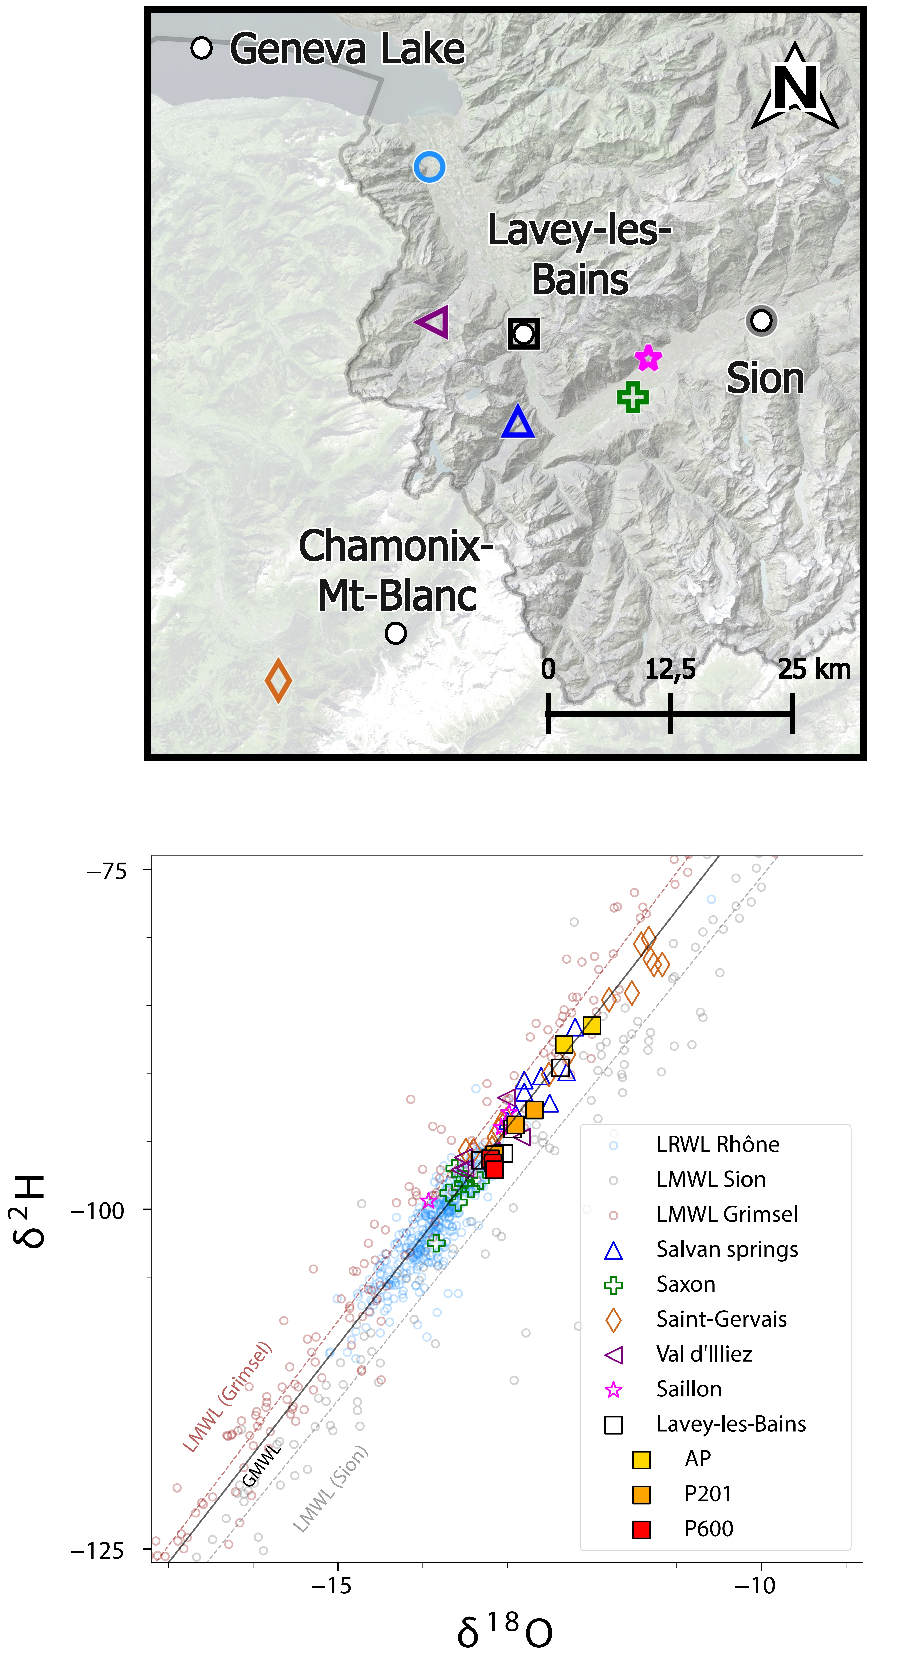
\includegraphics[height=0.55\textheight]{chapters/03_chap2/figures/figure_2.pdf}
\caption{
Geographic mapping of water sampling in the Lavey-les-Bains region (\textit{top}) and stable isotopic composition (\textit{bottom}): the isotopic signatures of all samples from various water sources, including local precipitations, river water, drinking water, and thermal springs, plot closely along the global meteoric water line (GMWL), bracketed by local meteoric water lines (LMWL) from Sion at \SI{482}{\meter} and Grimsel at \SI{1950}{\meter}.
This alignment indicates that the thermal waters of Lavey-les-Bains and other local water sources originate from recent meteoric water that has fallen in the Rhône valley and the Aiguilles Rouges massif.
Compared to Lavey-les-Bains, wells in Saint-Gervais-les-Bains and Val d'Illiez, which are believed to recharge in the same area as the Lavey-les-Bains' thermal waters \parencite{sonney2010groundwater}, indeed have similar isotopic composition as the thermal waters at P600. 
Furthermore, drinking water springs near the village of Salvan (Table~\ref{tabSI:stables_Salvan}), which range in altitude from \SI{900}{\metre} to \SI{1950}{\metre} in the supposed recharge area, display isotopic values that lie between those of P600 and AP.
Map sources: satellite imagery \parencite{swisstopo2024swissimage}; digital elevation model \parencite{swisstopo2024swissalti3D}; boundaries \parencite{swisstopo2024landesgrenzen}; EPSG:3035.}
\label{fig:stables}
\end{figure}



\subsubsection{Dissolved Gases}
Alternating between the P201 and P600 wells at Lavey-les-Bains, the mini-RUEDI system, which allows continuous on-site gas measurements, has collected over \num{100000} individual measurements for each gas (\ce{^4He}, \ce{^{40}Ar}, \ce{^{84}Kr}, \ce{N2}, \ce{O2}, \ce{CO2}, \ce{CH4}, and \ce{H2}) during four years of monitoring, revealing pronounced temporal and depth variations.
Particularly, the concentrations of \ce{CH4} and \ce{CO2} in P201 exhibit clear seasonal fluctuations that strongly correlate with patterns in electrical conductivity (Figure~\ref{fig:season}).
\ce{CH4} concentrations are reversely correlated with \ce{CO2} over time, with low \ce{CH4} concentrations correlating with low electrical conductivity measurements.
The \ce{CO2} and \ce{CH4} variations quantify in the range of \SI{25}{\percent}.
\ce{H2} also displays substantial seasonal variability, about \SI{75}{\percent}, typically lagging slightly behind the \ce{CO2} variations.
The rest of the gases show smaller (Kr and Ar) or no clear (\ce{O2}, and He) seasonal trend.
\ce{O2} was detected in both P201 and P600, but at very low concentrations (\SIrange{0.4}{2.7}{\umol\per\litre}).


\FloatBarrier % Ensure previous floats are placed before proceeding

\afterpage{% Delays the figure until the next page
\clearpage
\begin{figure}[p]
\begin{center}
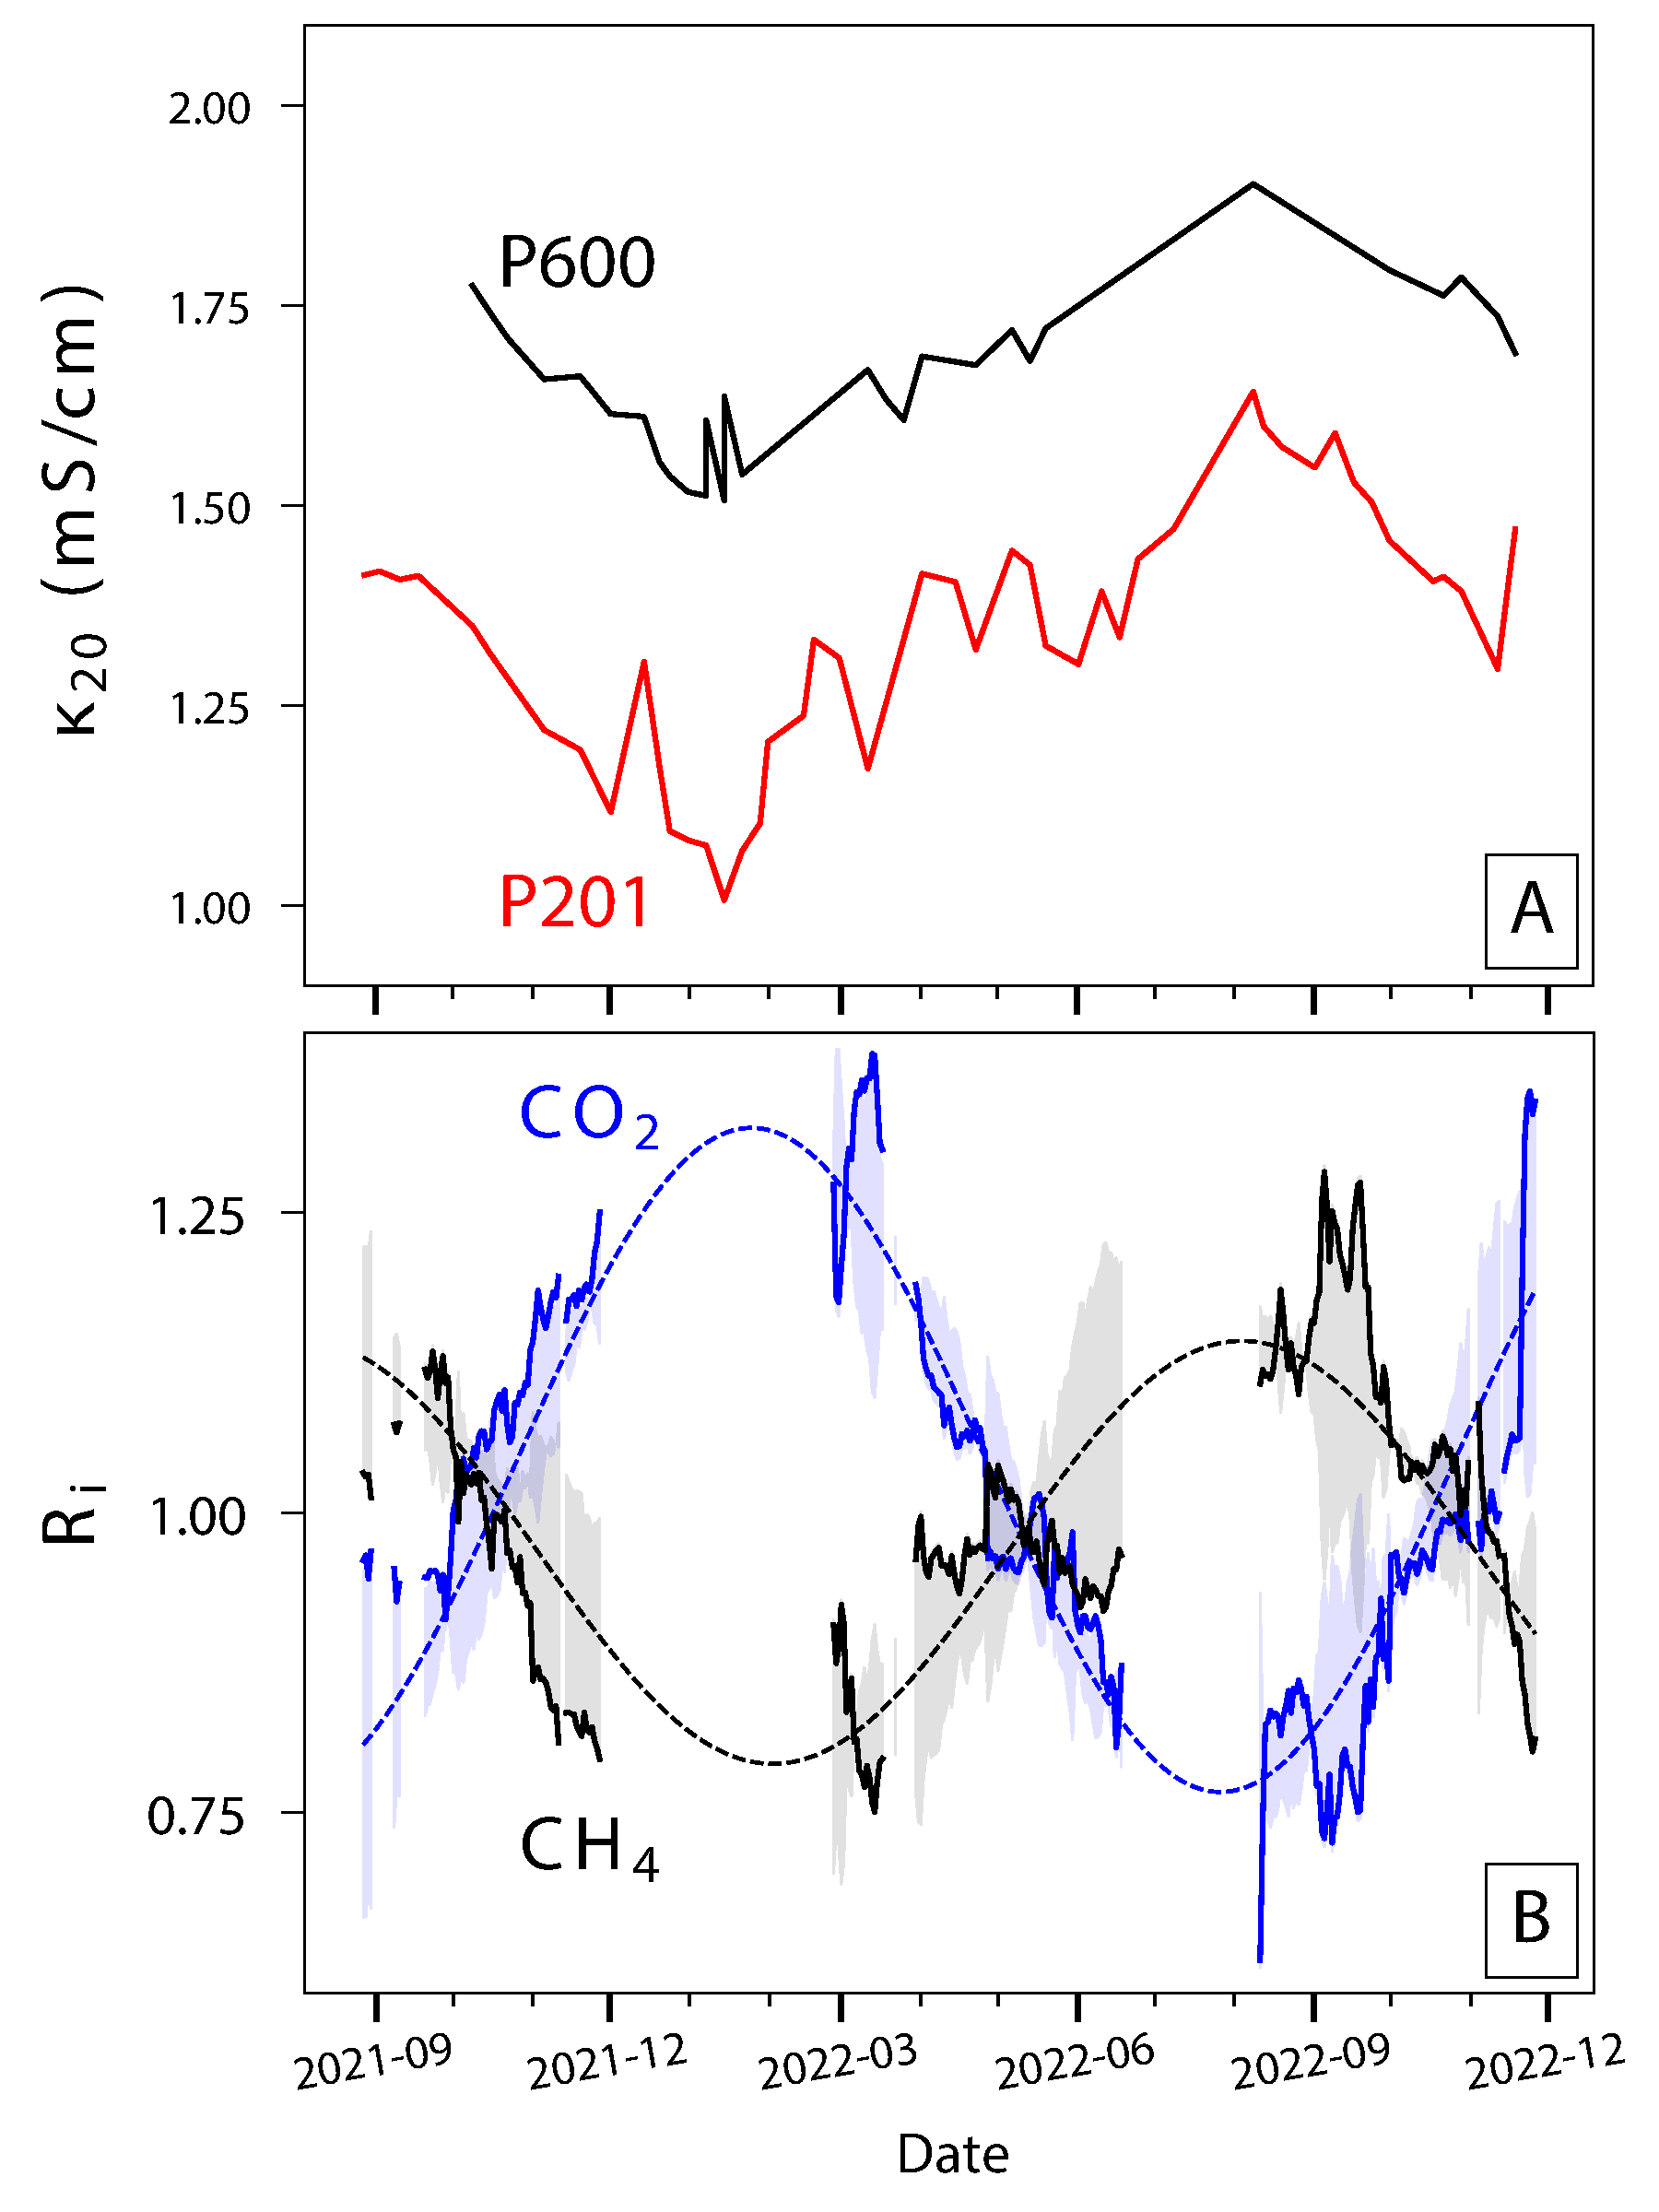
\includegraphics[width=0.6\textwidth]{chapters/03_chap2/figures/figure_1.pdf}
\end{center}
\caption{
\textit{A}: Weekly measurements of electrical conductivity (\SI{}{\milli\siemens\per\centi\metre}) for wells P600 (black) and P201 (red), highlighting seasonal variations.
Despite the clear offset, both curves appear to be temporally correlated. 
\textit{B}: Normalized partial pressures ($R_i$) of \ce{CO2} (blue) and \ce{CH4} (black) relative to \ce{N2} in well P201 (solid line).
The data shows daily averages of measurements taken with a time resolution of about \SI{10}{\minute}. 
The dotted line models the sinusoidal fluctuations over a period of \SI{365}{days}, with shaded areas indicating the deviation between the model and observed data.}
\label{fig:season}
\end{figure}
\clearpage
}

Due to technical constraints, seasonal trends of dissolved gases at well P600 could not be fully assessed, as data collection was limited to the period of approximately October through April each year when the spa pump was active.
As a result, the time series for P600 is incomplete, making it uncertain whether the dissolved gas concentrations at P600 exhibit seasonality similar to those observed in P201.
However, the electrical conductivity in P600 suggests a similar seasonal variability as in P201.

The concentrations of the geogenic gases (He, \ce{H2}, and \ce{CO2}) are similar between wells P201 and P600, indicating a uniform vertical ascent of deep terrestrial fluid components (Table~\ref{table:geochemistry}).
However, \ce{CH4} concentrations show a rather different behavior.
In well P201, \ce{CH4} concentrations are twice those measured in P600, suggesting that additional \ce{CH4}-enriched waters are introduced into the thermal system between \SI{200}{\metre} and \SI{500}{\metre}, resulting in the elevated levels observed (Table~\ref{table:geochemistry}).
Correlation analysis {(Figure~\ref{figSI:correlation})} of the data additionally shows that the more atmospheric gases \ce{N2} and Ar correlate strongly (0.81) with \ce{CH4} in well P201, further supporting additional isotopically enriched \ce{CH4} entering the system from a shallower aquifer. 
In contrast, \ce{CH4} correlates with \ce{CO2} in P600 (0.65), indicating for both geogenic sources from a deep aquifer. 

The results of the off-site copper tube gas analyses from the different wells at Lavey-les-Bains are largely consistent with the onsite miniRUEDI measurements, but also allowed the tritium content to be quantified (Tables~\ref{tabSI:noble_gases} and \ref{tabSI:isotope_ratios}).
The tritium content of all the thermal waters at Lavey-les-Bains is low (\SIrange{0.9}{1.4}{\TU}), with P600 being the lowest, while the surface well AP has a higher content of \SI{5.7}{\TU}.
The waters from P201, P280 and P600 show a clear enrichment of \ce{^{40}Ar} with \ce{^{40}Ar}/\ce{^{36}Ar} ratios around \SI{}{320} compared to surface well AP and control well E2, which have atmospheric-like ratios (close to 295.5).
All \ce{^3He}/\ce{^4He} ratios of the deep wells (\SIrange{1.5e-8}{2.8e-8}{}) show high enrichment of crustally generated \ce{^4He} (Figure~\ref{figSI:NeHe_plot}), whereas \ce{^{20}Ne}/\ce{^{22}Ne} ratios are atmospheric.

$\delta^{13}$C-\ce{CH4} values from the thermal waters at Lavey-les-Bains fall within the range of \SIrange{-16.4}{-4.1}{\permille} and $\delta^{2}$H-\ce{CH4} values within the range of \SIrange{17.4}{121.9}{\permille}, with P280 showing the heaviest isotopic signatures.
In contrast, $\delta^{13}$C-\ce{CH4} was clearly lighter at the surface well AP (\SI{-28.4}{\permille}).
The heavy isotopic signatures in deeper layers are accompanied by \ce{CH4} to ethane ratios of \SIrange{27.6}{254.4}{}.
Typically, biogenic \ce{CH4} production features much higher ratios, often exceeding 1000, and is associated with lighter $\delta^{13}$C-\ce{CH4} values \citep{whiticar1999carbon, faber2015geochemical}.
The relatively low ratios observed here, along with the \ce{CH4} isotopic data being enriched, indicate that the \ce{CH4} in this thermal system predominantly originates from abiotic, crustal sources (Figure~\ref{figSI:CD_plot}).
At or near the surface, however, there is an addition of biologically produced (i.e., isotopically light) \ce{CH4}.
Remarkably, the $\delta^{13}$C-DIC signature remains nearly constant from the deep to the surface of the thermal system, ranging from \SIrange{-10.3}{-11.4}{\permille}.
This consistency across the vertical profile of the aquifer implies a stable and common \ce{CO2} source, most likely rock-related.

\subsubsection{Volatile Fatty Acids}
In addition to the geochemical and gas data, concentrations of short-chain volatile fatty acids (VFAs), specifically acetate and formate, were measured in all sampled wells (Table~\ref{table:microbiology}).
Acetate concentrations ranged from \SIrange{0.7}{2.8}{\umol\per\litre}, while formate concentrations varied between values below the detection limit ($< \SI{0.5}{\umol\per\litre}$) and \SI{2.7}{\umol\per\litre}.


\subsection{Microbiological data}
We investigated potential depth-related changes in situ microbial communities by sampling microbial biomass in boreholes AP, P201, P280, and P600.
To explore seasonal variations in response to winter (low electrical conductivity and \ce{CH4} concentration, high \ce{CO2} concentration), and summer conditions (high conductivity and \ce{CH4} concentration, low \ce{CO2} concentration), boreholes P201 and P600 were sampled on three different dates.

\begin{table*}[ht]
\caption{Microbiological quantification in the three main deep wells of Lavey-les-Bains and the surface well AP.}
\label{table:microbiology}
\centering
{\footnotesize
\renewcommand{\arraystretch}{1.2}
\resizebox{\textwidth}{!}{%
\begin{tabular}{l|c|ccc|c|ccc}
\toprule
\multirow{2}{*}{Borehole}   &   AP &   \multicolumn{3}{c|}{P201}    & P280   & \multicolumn{3}{c}{P600}                \\
    & \SI{28}{\metre} & \SI{201}{\metre} & \SI{201}{\metre} & \SI{201}{\metre}
    & \SI{276}{\metre} & \SI{516}{\metre} & \SI{516}{\metre} & \SI{516}{\metre} \\
\midrule
\multicolumn{9}{c}{\textbf{Microbiology}} \\
\midrule
Sampling date Microbiology  & 25.10.21 & 20.09.21 & 25.10.21 & 11.01.22   & 20.09.21 & 26.04.21 & 25.10.21 & 11.01.22 \\
Acetate [\SI{}{\umol\per\litre}] & 0.7     & 1.8 & 2.1 & 2.8 & 1.7 & 2.2 & 0.9 & 2.5 \\
Formate [\SI{}{\umol\per\litre}] & $< 0.5$ & 2.7 & 2.5 & 1.1 & 2.1 & 1.2 & 0.9 & 1.0 \\
16S bac [\SI{}{\copies\per\milli\litre}]  & \num{170}  & \num{5369} & \num{12357}  & \num{3094}  & \num{4253} & \num{1283} & \num{156}  & \num{78}     \\
\textit{mcrA} [\SI{}{\copies\per\milli\litre}] & 0.1  & 0.1  & 0.4  & 0.2 & 0.9  & 0.4  & 1.0 & 0.0 \\
Archaeal Shannon index                &  2.2 & 0.6  & 0.7  & 1.7 & 0.3  & 2.3  & 2.4 & 2.2 \\
Bacterial Shannon index               &  3.5 & 1.2  & 0.7  & 3.0 & 1.4  & 2.0  & 2.9 & 2.7 \\
Bacterial Inv. Simpson index          & 17.4 & 1.5  & 1.3  & 3.8 & 1.8  & 4.0  & 5.9 & 8.5 \\
\midrule
\end{tabular}%
}
}
\end{table*}


\subsubsection{Microbial abundance}
Bacteria and Archaea abundances based on 16S rRNA gene copy numbers range between \SIrange{78}{12357}{\copies\per\milli\litre} and \SIrange{3}{350}{\copies\per\milli\litre}, respectively, with P201 and P280 having the highest abundances (Table~\ref{table:microbiology}).
While the upper range is comparable to samples taken from deep boreholes in Scandinavia, most samples show considerably lower biomass \citep{itavaara2011characterization, bomberg2015active}.

Bacteria-to-Archaea ratios (BAR) are in the range of \SIrange{5.4}{64.2}{} in the sampled thermal system of Lavey-les-Bains.
Despite the high temperatures ($>\SI{45}{\celsius}$) that reportedly lead to dominance of Archaea \citep{lagostina2021interactions}, Bacteria dominate even at \SI{65}{\celsius}.
We additionally detected ammonia oxidizing Archaea (AoA) in the surface well AP and the intermediate wells P201 and P280, with abundances ranging between \SIrange{4.9}{37.6}{\copies\per\milli\liter}.
By contrast, methanogenesis genes (\textit{mcrA}) were almost not detected (\SIrange{0}{0.9}{\copies\per\milli\liter}).

\subsubsection{Spatiotemporal trends in microbial community structure}
Assessments at the zero-radius operational taxonomic unit (ZOTU) level indicate a clear, depth-related zonation of microbial communities.
Microbial community diversity (Shannon Index) and evenness (Inverse Simpson Index) are highest at the surface (AP), decrease at intermediate depths (wells P201 and P280), and then increase again in the deepest layer (P600) (Table~\ref{table:microbiology}).
A Principal Coordinates Analysis (PCoA; Figures~\ref{figSI:PCoA_arc} and \ref{figSI:PCoA_bac}) shows clear separations in microbial community fingerprints between the three depth layers, with the principal axes explaining up to \SIrange{50}{90}{\percent} of the observed variation.
No clear seasonal changes in diversity or evenness were apparent in P201 or P600.

The clear depth-related changes in microbial communities at the ZOTU-level are mirrored in major taxonomic changes (Figure~\ref{fig:microbio}).
These depth-related changes are far greater than temporal changes in microbial communities throughout the year.
At the surface (AP), bacterial communities are dominated by Proteobacteria (Hyphomicrobiales, Nitrosomonadales, Others, including Burkholderiales, Rhodobacterales, and Rhodospirillales), followed by Actinomycetota (Acidimicrobiales), and lower, yet significant contributions of Patescibacteria (Nomurabacteria), Acidobacteriota, and Actinobacteria.
In contrast, at intermediate depths (P201 and P280), the bacterial community composition is very clearly dominated by Nitrospirota (Nitrospirales), with minor contributions of Nitrosomonadales and Patescibacteria (Jorgensenbacteria).
Bacterial communities in the deepest layer (P600) are again very different, with Thermales and Thermodesulfobacteriota dominating, followed by Aquificota, Nitrosomonadales, Acidobacteriota and Thermodesulfobacteriota as minor groups.

Archaeal communities display similarly pronounced depth-related taxonomic changes.
While AP is dominated by Thaumarchaeota (Nitrosopumilales and SAGMCG) and to a lesser degree Woesearchaeota, intermediate depths (P201 and P280) contain on average $> \SI{85}{\percent}$ Micrarchaeota.
The deepest samples harbor the most complex archaeal communities, with major contributions of Bathyarchaeota.
The latter include a novel, deeply-branching class-level group (Figure~\ref{figSI:MCG31}) with only about \SI{80}{\percent} 16S rRNA gene sequence similarity to other Bathyarchaeota based on Basic Local Alignment Search Tool (BLAST) analyses. 

Microbial metabolic profiling, inferred from the phylogenetic composition, reveals a clear transition in metabolic strategies with depth (Tables~\ref{tabSI:tax_arc_1}-\ref{tabSI:tax_arc_2} and \ref{tabSI:tax_bac_1}-\ref{tabSI:tax_bac_2}).
At the surface (AP), the community is essentially aerobic and dominated by ZOTUs belonging to heterotrophs (\textit{Ilumatobacteraceae}, \textit{Reyranella}; \cite{asem2018ilumato, cui2017reyranella}), methanotrophs (\textit{Methylocystis}, \textit{Methylotenera}; \cite{afshin2021methylotenera, bowman2015methylocystis}), as well as other methylotrophs (\textit{Methyloversatilis}; \cite{doronina2014methyloversatilis}).
At intermediate depths (P201 and P280), the bacterial community becomes clearly dominated by \textit{Dissulfurispiraceae} (Nitrospirales), suggesting sulfur disproportionation as the primary energy source \citep{umezawa2021dissulfurispira}.
By contrast, the dominant archaeal phylum (Micrarchaeota) is believed to consist of aerobic or anaerobic fermentative heterotrophs with potentially symbiotic lifestyles \citep{kadnikov2020micrarachaeota, chen2018micrarchaeota, sakai2022micrarchaeota}.
A striking difference in the deepest layer (P600), is the prevalence of ZOTUs belonging to taxa that include known thermophiles and hyperthermophiles.
The dominant ZOTUs belong to heterotrophs (\textit{Thermus}, \textit{Thermoanaerobaculum}, \textit{Thermotogae}, Bathyarchaeota, Micrarchaeota, Aenigmarchaeota) and potential sulfate- or iron-reducing \ce{H2}-oxidizers (\textit{Hydrogenobacter}, \textit{Geothermobacterium}, \textit{Sterolibacteriaceae}) \citep{williams1995thermus, mori2014thermodesulfobacteriaceae, zeytun2011hydrogenobacter, kadnikov2020micrarachaeota, boden2017sterilo, kashefi2002geothermobacterium, garrido2023enrichment, losey2020thermoanaerobaculum}.


\FloatBarrier % Ensure previous floats are placed before proceeding

\afterpage{% Delays the figure until the next page
\clearpage
\begin{sidewaysfigure} % Rotates the figure to landscape mode
\begin{center}
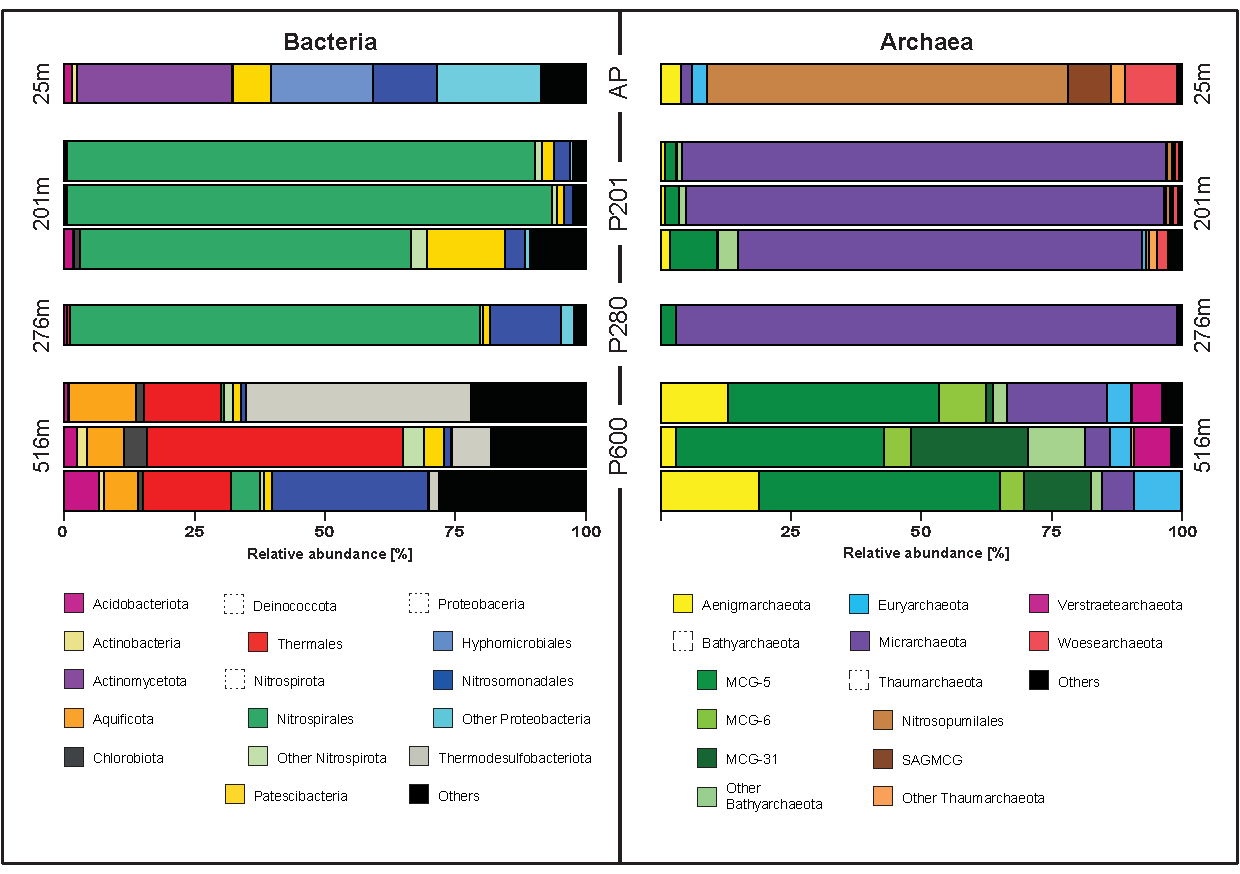
\includegraphics[width=0.8\textheight]{chapters/03_chap2/figures/figure_3.pdf} % Adjust width
\end{center}
\caption{Analysis of the relative abundance of microbial communities based on 16S rRNA gene sequencing from Lavey-les-Bains wells. 
Bacterial (\textit{left}) and archaeal (\textit{right}) community compositions at the phylum level; predominant phyla (dashed squares) are further categorized by their dominant orders to detail the community structure.}
\label{fig:microbio}
\end{sidewaysfigure}
\clearpage
}


%%%%%%%%%%%%%%%%%%%%%%%%%%%%%%%%%%%%%%%%%%%%%%%%%%%%%%%%%%%%%%%%%%%%%%%%%%%%%%%%%%%%%%%%%%%%%%%%%%%%%%%%%%%%

\section{Discussion}
\subsection{Hydrological Dynamics and Isotopic Variations in Lavey-les-Bains}
The hydrological dynamics of the Lavey-les-Bains system are driven by mixing of deep, ancient groundwater with shallower, more recently infiltrated water, as revealed by the geochemical and isotopic data.
Water from P600, characterized by depleted stable water isotopes and low tritium levels, suggests minimal recent recharge and prolonged residence times within the aquifer, which is consistent with a strong geothermal overprint on the groundwater \citep{sonney2009numerical, vuataz1982hydrogeologie}.
In contrast, the enriched stable isotopes and higher tritium levels in shallower waters of P201 and P280 suggest more recent infiltration, likely from the Rhône valley and surrounding mountains.
The presence of low-altitude infiltrated water at significant depth is further supported by the noble gas concentrations measured in E2, indicating recharge between \SIrange[range-phrase = { and }]{500}{1000}{\meter} of altitude.

This seasonally varying mixing of geothermal deep groundwater with a shallow groundwater component is clearly reflected in the electrical conductivity and dissolved gas concentrations throughout the system.
Deep well P600, which taps water that has circulated through the fractured gneiss of the Aiguilles Rouges massif for millennia, consistently shows the highest conductivity and elevated \ce{^4He} concentrations.
Together with the \ce{^{40}Ar}/\ce{^{36}Ar} ratio higher than atmospheric, these features indicate prolonged water-rock interaction and geothermal heating within the crust \citep{torgersen1982helium}.

In contrast, the shallower wells P201, P280 show more pronounced seasonal variations.
These variations, particularly in conductivity and gas concentrations, most likely arise from a piston effect that is caused by the annual snowmelt recharge pulse, which exerts hydraulic pressure on deeper groundwater, forcing it upward into the shallower parts of the system.
This phenomenon, often referred to as the "old groundwater paradox", results in the discharge of older, more chemically evolved groundwater during periods of increased surface recharge \citep{schilling2021quantifying, mcdonnell2003where, kirchner2003double}.

The higher hydraulic pressure during the summer affects not only the deep, old water component but also the abiotic \ce{CH4}-bearing component.
This additional component enters the Lavey-les-Bains wellfield between the depths of \SI{200}{\metre} and \SI{500}{\metre}, leading to elevated concentrations of \ce{CH4} during late summer. 
These \ce{CH4} concentrations, which are anticorrelated with \ce{CO2}, provide insight into the biogeochemical processes in the subsurface.
The data suggest that \ce{CH4} production is driven by the upward migration of deep, thermogenic \ce{CH4}, while \ce{CO2} dynamics may be influenced by abiotic processes occurring within the aquifer.

While the high $\delta\ce{^{13}C}$-\ce{CH4} signatures (\SIrange{-16.4}{-4.1}{\permille}) in intermediate and deeper layers could indicate a deep thermogenic origin or oxidative enrichment of \ce{CH4} initially produced by aceticlastic methanogenesis (Figure~\ref{figSI:CD_plot}), $\delta\ce{^{2}H}$-\ce{CH4} values provide a clearer picture.
The highly positive \ce{^2H}-values, ranging from \SIrange{17}{122}{\permille}, are among the highest reported and point to oxidative fractionation of a deep, thermogenic \ce{CH4} pool \citep{etiope2011homorod}.
Given that we did not recover 16S rRNA gene sequences of known \ce{CH4}-cycling microorganisms in the deeper layers and that \textit{mcrA} gene copies were close to the detection limit in all samples, an abiogenic oxidation process—possibly high-temperature chemical oxidation by iron oxides seems likely \citep{etiope2011homorod}.
By contrast, the more negative $\delta\ce{^{13}C}$-\ce{CH4} in the shallow layer (AP) indicate a significant contribution from a shallow, most likely biogenic, \ce{CH4} source.

While local pumping operations can potentially affect groundwater mixing patterns, their effects appear to be limited to areas of sharp, short-term changes, such as those observed in conductivity measurements from December 2021 to January 2022 (Figure~\ref{fig:season}).
The seasonal variability observed in both P600 and P201 appears to be primarily driven by natural hydraulic gradients resulting from seasonal discharge dynamics (e.g., snowmelt) rather than pumping regimes optimized for the seasonal needs of the spa.
To better distinguish between natural and induced mixing processes, a more rigorous monitoring scheme, including more frequent stable isotope and tritiogenic sampling, would be needed.
Such an approach would provide clearer insights into the temporal and spatial dynamics of water mixing in the Lavey-les-Bains thermal system.


\subsection{Drivers of in situ Microbial Communities}
The microbial community structure in the Lavey-les-Bains hydrothermal system shows a clear depth zonation, with distinct communities in the surface, intermediate and deep layers.
The surface communities appear to be strongly influenced by surface and shallow aquifer processes, as indicated by the dominance of aerobic heterotrophs and methylotrophs, reflecting adaptation to aerobic conditions.
At intermediate depths, wells P201 and P280 are dominated by \textit{Dissulfurispira}, which includes sulfur-disproportionating microorganisms, and the enigmatic archaeal order Micrarchaeota, associated with symbiotic aerobic and anaerobic heterotrophic lifestyles \citep{umezawa2021dissulfurispira, chen2018micrarchaeota, sakai2022micrarchaeota, kadnikov2020micrarachaeota}.
The very limited diversity, i.e. about \SI{75}{\percent} of bacterial reads and over \SI{80}{\percent} of archaeal reads consistently belonged to the same ZOTUs of Nitrospirales and Micrarchaeota, respectively, suggests that environmental conditions, such as temperatures near the mesophile-thermophile transition and fluctuating redox conditions, may support only a narrow range of microorganisms at these detphs.
Interestingly, microbial diversity increases again at P600, which is dominated by ZOTUs potentially involved in anaerobic fermentative degradation of organic matter and anaerobic respiration of \ce{H2}.
Notably, many of these ZOTUs belong to thermophilic taxa, suggesting that this switch to an organotrophic microbial community may be related to the heat-activated bioavailability of fossil organic matter in this layer \citep{lagostina2021interactions}.

The large community shift between intermediate and deep layers indicates that temperature is a key factor in structuring microbial communities.
Even for those taxa that are present in significant abundance across shallow, intermediate, and/or deep layers (e.g., Patescibacteria, Nitrosomonadales, Micrarcheia, Euryarchaeota; Figure~\ref{fig:microbio}), the dominant ZOTUs consistently differ between these layers (Tables~\ref{tabSI:tax_arc_1}-\ref{tabSI:tax_arc_2} and \ref{tabSI:tax_bac_1}-\ref{tabSI:tax_bac_2}).
This clear separation of microbial communities between different temperature settings, despite hydrological connectivity, argues for the existence of a significant planktonic microbiome.
However, it is more likely that the vast majority of microorganisms recovered grow on rock surfaces and were dislodged as a result of increased fluid flow caused by fluid pumping prior to sampling.

The drastic change in microbial communities despite only about \SI{10}{\celsius} increase in measured temperatures between P201 and P280 (\SIrange{51.8}{53.2}{\celsius}) and P600 (\SIrange{62.9}{63.6}{\celsius}) is striking and suggests that even small changes in temperature can greatly affect microbial community structure in subsurface aquifers.
One explanation is that the upper temperature limit of in situ mesophilic microorganisms is higher than that of most mesophilic microorganisms under laboratory conditions (about \SI{45}{\celsius}), and lies between the temperatures of P201/P280 and P600.
This would explain the community shift towards dominance of thermophilic taxa at P600.
In addition, temperature fluctuations may play a role: although measured temperatures remained relatively stable (within \SI{4}{\celsius}, Figure~\ref{figSI:EC_vs_temp}) from 2021 to 2024, historical records indicate a temperature decrease in P201 since the early 2000s \citep{sonney2009numerical}.
Such temperature fluctuations, which cross thermal thresholds for in situ microorganisms, may also have contributed to the reduced taxonomic diversity observed in P201/P280.

In contrast, we do not find evidence for an important role of fluid chemistry in driving microbial communities.
Despite strong seasonal fluctuations in conductivity, \ce{CO2}, and \ce{CH4}, potential temporal responses in microbial communities to changes in these variables are overshadowed by changes in relation to temperature.
This temporal stability of microbial communities over the study period could have several reasons.
For instance, in situ microbial communities could be resilient to fluctuating conductivities and according mixing ratios of deep and shallow groundwaters and not be limited by \ce{CO2} or \ce{CH4} availability \citep{lever2015life, hoehler2013microbial}.
The importance of such resilience would match the long generation times of subsurface microorganisms, which can range from months to years \citep{joergensen2011deep}.
Slow metabolic and growth rates may require these organisms to persist short-term changes in geochemistry as observed with respect to conductivity, \ce{CO2}, and \ce{CH4}.
In addition, concentrations of other, potentially important in situ electron donors (e.g., organic acids, ammonium, \ce{H2}) and acceptors (e.g., \ce{O2}, \ce{SO4^{2-}}) are remarkably consistent over time and across depths sampled.

In the geological context of the Lavey-les-Bains site, the lithological profiling shows minimal variation between the three boreholes, with quartz-feldspar making up the majority of the bedrock composition, consistently above \SI{70}{\percent}, supplemented by varying amounts of chlorite gneiss, mica and biotite gneiss \citep{swisstopo2024lavey1}.
From about \SI{100}{\meter} to \SI{596}{\meter}, the composition ranges are approximately as follows: quartz-feldspar (\SIrange{70}{85}{\percent}), chlorite gneiss (\SIrange{2}{25}{\percent}), mica (\SIrange{1}{5}{\percent}), and biotite gneiss (\SIrange{3}{25}{\percent}), with the remaining components making up \SIrange{1}{4}{\percent}.

Despite these differences, there does not appear to be a significant effect of this mineralogical diversity on the microbial communities within the wells.
For example, the similarity between the microbial communities in P201 and P280 remains high even though these wells exhibit differences in secondary mineral content.
This observation suggests that while lithological factors may influence microbial habitats to some extent, they are not the primary drivers of the microbial community structures observed in these wells.
Instead, it appears that temperature variations at different depths play a critical role in shaping these communities.
The water flowing into the boreholes from fractures at different depths introduces an element of inconsistency that prevents absolute comparisons of mineral content between specific boreholes.
Consequently, our results indicate that depth-related thermal variations are the primary determinants of the observed vertical zonation of microbial communities within the Lavey-les-Bains underground aquifer.

\section{Methods}
\subsection{Study site}
The Lavey-les-Bains site (Vaud, Switzerland) is characterized by its extensive thermal system, evidenced by over 30 boreholes that span depths ranging from 10 to over \SI{500}{\meter} depth.
This array of boreholes provides the assessment of the terrestrial subsurface environment at various depths.
According to the current conceptual model, thermal waters traverse the fractured crystalline gneiss of the Aiguilles Rouges massif---a geological formation spanning the French and Swiss Alps---over several millennia (\SIrange{8000}{30000}{\year}; \cite{sonney2009numerical, bianchetti1994hydrogeologie}).
These waters reach estimated reservoir temperatures of about \SIrange{110}{120}{\celsius} \citep{sonney2009numerical, wanner2019quantification}.
Bore logs of various wells \citep{swisstopo2024lavey1} have identified Quaternary sediments in the initial \SI{40}{\meter} followed by chlorite schist. 
Below this, the geology predominantly features alternating strata of chlorite gneiss, biotite gneiss (migmatitic), and orthogneiss, with a significant composition of quartz-feldspar rocks.

Central to our investigation are three deep wells---P201, P280, and P600---spaced \SIrange{40}{200}{\meter} apart (Figure~\ref{figSI:map_Lavey}).
These wells tap into different strata to supply thermal water to the local spa facility.
P201 and P600, with depths of 201 and \SI{516}{\meter} and water temperatures of \SI{51}{\celsius} and \SI{64}{\celsius}, respectively, serve seasonal heat demands of the spa during summer and winter. 
P280, at \SI{276}{\meter} and \SI{53}{\celsius}, acts as a supplementary source to cover peak usage periods.

Additionally, our analysis includes a non-producing surface well AP (\SI{28}{\meter} depth) within the wellfield of Lavey-les-Bains and a deep well E2 (Epinassey, Valais, \SI{216}{\meter} depth) outside the thermal system. 
The AP well provides insights into the passive mixing of surface waters from the Rhône valley plain with ascending deep groundwater, whereas the E2 well serves as proxy to understand recharge at depth.

\subsection{Data acquisition and geochemical sampling}
Electrical conductivity measurements and chemical analyses were provided by Alpgeo Sarl, using a WTW device.
For comprehensive geochemical analysis, water samples were sent to an external laboratory adhering to standard DIN/ISO/SN methods.

We compiled stable water isotopes from different studies \citep{vuataz1982hydrogeologie,sonney2009numerical,sonney2010groundwater} and by referring to the BDFGeotherm database from CREGE \citep{sonney2010database}.
We supplemented these data with our stable water isotope measurements for the regions of Salvan and Lavey-les-Bains regions, carried out at Eawag using a cavity ring-down laser spectrometer (Picarro) with nitrogen carrier gas (Table~\ref{tabSI:stables_Salvan}). 
The typical measurement uncertainties are \SI{0.05}{\permille} for $\delta$\ce{^{18}O} and \SI{0.5}{\permille} for $\delta$\ce{^{2}H}.
Additional regional data were sourced from the Global Network of Isotopes in Precipitation (GNIP) and the Global Network of Isotopes in Rivers (GNIR) managed by the IAEA, covering locations such as Grimsel, Sion, and Rhône--Porte du Sex \citep{iaea2024GNIP, iaea2024GNIR, naqua2024isot}.

Continuous on-site dissolved gases measurements were conducted using a gas-equilibrium membrane-inlet mass spectrometer (miniRUEDI), specially adapted to withstand the harsh conditions of long-term monitoring in thermal waters \citep{giroud2023new, brennwald2016portable}.
This system enabled the real-time analysis of eight gases (\ce{H2}, \ce{CH4}, \ce{N2}, \ce{O2}, \ce{^{40}Ar}, \ce{CO2} measured on the Faraday cup, and \ce{^4He} and \ce{^{84}Kr} on the multiplier detector), with a resolution of approximately \SI{10}{\minute}.
Data filtering was employed using water temperature as a threshold to ensure measurements were only recorded when pumps were active, ensuring data relevance and accuracy.

Additionally, discrete water samples were collected in copper tubes for off-site laboratory analysis at ETH Zurich \citep{beyerle2000mass}.
These analyses focused on noble gases concentrations (He, Ne, Ar, Kr, Xe) and isotopic ratios (\ce{^3He}/\ce{^4He}, \ce{^{20}Ne}/\ce{^{22}Ne}, \ce{^{40}Ar}/\ce{^{36}Ar}), as well as tritium concentration (\ce{^3H}) to provide further insights into the age and origins of the water sources.

Dissolved inorganic carbon samples ($\delta$\ce{^{13}C}-\ce{CO2}) were taken in the field in Eppendorf tubes without headspace, transferred to helium-flushed borosilicate tubes prefilled with phosphoric acid for \ce{CO2} release, and analyzed using a MAT 253 isotope ratio mass spectrometer (IRMS, Thermo Fisher Scientific) \citep{vandijk2018oxygen}.

\ce{CH4} samples for $\delta$\ce{^{2}H}-\ce{CH4} and $\delta$\ce{^{13}C}-\ce{CH4} isotopic analysis were collected in glass bottles, which were then treated with NaOH pellets to stop microbial activity and crimped to eliminate headspace, ensuring no gas exchange. 
Isotopic ratios of \ce{CH4} were analyzed from the induced headspace using trace gas IRMS for the $\delta$\ce{^{13}C} \citep{thomas2019lateral} and gas chromatography combustion IRMS following internal protocols for $\delta$\ce{^{2}H} at Kastanienbaum, Eawag. 
VFAs were measured by 2D-ion chromatography \citep{glombitza2014vfas}.

Isotopic results are noted in the standard $\delta$-notation relative to Vienna PeeDee Belemnite (VPDB) for carbon isotopes and to Vienna Standard Mean Ocean Water (VSMOW) for hydrogen and oxygen isotopes.


\subsection{Sampling and DNA Extraction}

Water samples (\SIrange{2}{5}{\litre}) were collected in sterilized glass bottles from various thermal water wells at Lavey-les-Bains.
For the surface well AP, a standard Niskin bottle used for water column sampling in lakes and oceans was applied to sample the well. 
To determine the level of contamination, autoclaved ultra-filtered water was filled on the field into the same type of glass bottle to serve as a negative control (NTC).
Both water samples and NTCs were immediately transported on ice to the laboratory at ETH Zurich to ensure preservation and stability for subsequent processing.

In the laboratory, water samples and NTCs were filtered within a portable nitrogen glove box to minimize potential (lab) air contamination.
This process involved the use of filter towers (Nalgene™ Rapid-Flow™ Sterile Disposable Filter Units, ThermoFisher) with \SI{0.1}{\micro\metre} polyethersulfone (PES) filters.
\SI{0.1}{\micro\metre} filters were selected in order to sample the entire fraction of the microbial communities (Figure~\ref{figSI:filter_comp}).
After filtration, the PES filters were carefully removed, placed into sterilized falcon tubes, and immediately stored at \SI{-80}{\celsius} to preserve the integrity of potential microbial DNA until extraction.

The DNA was extracted under strict conditions of a ductless fume hood within a clean lab at ETH Zurich to prevent contamination, especially given the expected low biomass in the samples.
The extraction protocol used was adapted from the Lysis Protocol I detailed by Lever et al. \citep{lever2015modular}, which was specifically tailored for low biomass samples (Supplementary Information for details).
The DNA samples were quantified using quantitative polymerase chain reaction (qPCR; \cite{lever2015modular, deng2022qpcr, meier2024qpcr}).

\subsection{DNA sequencing and bioinformatics}
We utilized archaeal primers ARC519F and ARC915Rmod \citep{soerensen2006stratified, cadillo2006vertical}, and bacterial primers S-D-Bact-0341-b-S-17 and S-D-Bact-0785-a-A-21 for 16S rRNA gene amplification \citep{herlemann2011trasitions}.
PCR products were barcoded and prepared for sequencing using a published workflow \citep{han2020eutrophication}. 
The sequencing was performed on a MiSeq Personal Sequencer (Illumina, San Diego, CA) using the 600PE kit, incorporating a \SI{10}{\percent} PhiX spike to ensure quality control across the sequencing run.

A comprehensive data preparation protocol is detailed in the Supplementary Information, which outlines the software applications used, the versions, the parameters applied, and details on reads and samples that were excluded from analysis.

Sequences from known contaminant organisms were searched in the samples from Lavey-les-Bains, and they were not significant for the identified microbial communities \citep{salter2014reagent, sheik2018identification}.
In addition, the most abundant taxa (mostly Proteobacteria) from negative template controls (NTCs) and extraction blanks (EBs) were compared with the samples from the Lavey-les-Bains wells, and they were not found to contribute significantly to the identified communities.

\subsection*{Data availability}
Geochemical data (hydrochemistry, noble gas measurements, and mini-RUEDI measurements) are available in the Supporting Information.
All sequences of this study are freely available on the GenBank with accession code SUB14782819.
Maps were generated by QGIS (v3.32.0).

\section{Supplementary Information}
See Appendix \ref{ch:appendix_ch2}.